\documentclass[conference]{IEEEtran}

\usepackage{cite}

\ifCLASSINFOpdf
  \usepackage[pdftex]{graphicx}
\else
  \usepackage[dvips]{graphicx}
\fi

%\hyphenation{op-tical net-works semi-conduc-tor}

\begin{document}

\title{OpenPowerQuality: An Open Source Framework for Power Quality Collection, Analysis, Visualization, and Privacy}

\author{\IEEEauthorblockN{A. Christe, S. Negrashov, P. Johnson}
\IEEEauthorblockA{Deptartment of Information and Computer Sciences,  
University of Hawaii at Manoa\\
Email: (achriste, sin8, johnson)@hawaii.edu}
}

\maketitle

\begin{abstract}
As power grids transition from a centralized distribution model to a distributed model, maintaining grid stability requires real-time power quality (PQ) monitoring and visualization.  As part of the Open Power Quality (OPQ) project, we designed and deployed a set of open source power quality monitors and an open source cloud-based aggregation and visualization system built with the utility customer in mind. Our aim is to leverage a flexible privacy model combined with inexpensive and easy to use PQ meters in order to deploy a high density power quality monitoring network across the Hawaiian islands. In this paper we describe OPHub, a privacy focused open source PQ visualization along with results of a small scale deployment of our prototype PQ meter across the island of Oahu. Our results demonstrate that OPQ can provide useful power quality data at an order of magnitude less cost than prior approaches.
\end{abstract}

\begin{IEEEkeywords}
Power Quality, Smart Grid, Data Visualization, Privacy, Open Source Hardware, Open Source Software, Distributed Power Generation, Wireless Sensor Network
\end{IEEEkeywords}

\IEEEpeerreviewmaketitle

\section{Introduction}
As power grids transition from a centralized distribution model to a distributed model, maintaining a stable grid requires fine grained knowledge of how distributed renewables are affecting the state of the grid. Monitoring PQ on a distributed generation smartgrid requires a consumer level distributed sensor network. How do we visualize power quality (PQ) on the power grid scale using data gathered from residential utility customers while maintaining their privacy?

To answer this question, we developed and deployed an open source hardware and software system with a flexible privacy model focused on consumer level monitoring across Oahu. 

Our system is able to display PQ at both the consumer level and the grid level. At its core is a visualization algorithm that uses a quadtree based map in order to display PQ data without sacrificing users' privacy.

In late 2014 we performed a pilot study to test the feasibility of our hardware and software system. Data collected during this study showed strong correlations between PV production and daily voltage trends. We demonstrated that a grid wide view allows us to determine if PQ events take place at the consumer level or at the grid level. We  able to maintain the privacy of our users by allowing them to choose a privacy profile that they were most comfortable with.

Finally, we could produce these boxes for under \$100 each. This is roughly an order of magnitude cheaper than other power quality monitoring equipment and is better suited for our applications.

\section{Privacy}
NIST describes privacy as one the main areas of focus and concern when implementing smart grid technologies\cite{p:kursawe_privacy_friendly_2011} and specifically proposes using ``privacy by design" as an ideal approach. The White House Big Data paper\cite{whitehouse} points out that privacy can be compromised even with perfect security and must be included as another layer and maintained on top of security. Baumeister \cite{baumeister2010literature} mentions that smart grid technologies should "motivate and include consumers". For these reasons, we decided to make privacy a top design goal for our project.

All data is collected on our servers, but identifiable information is not included by default. A user has the ability to decide if they alone will use their data or if they would like to share anonymized data with the community. With every user that decides to share their data, our knowledge of the state of the grid improves.

Baumeister\cite{baumeister2010literature} describes the importance of anonymizing data and the attack vectors that can be made against non-anonymized data. We do not share identifying information publically and strip as much superfluous information as possible.

When visualizing PQ data, we give the user the ability to select the granularity of their data collection device's location. We achieve this by using a custom quad-tree based map that is described in subsequent sections.


\section{Visualisation}
We designed and built an open source web application, OPQHub, that provides local and global displays of PQ data. Our service collects, aggregates, and analyzes PQ data from a set of distributed PQ meters (figure \ref{fig:opqhub}).

\begin{figure*}
  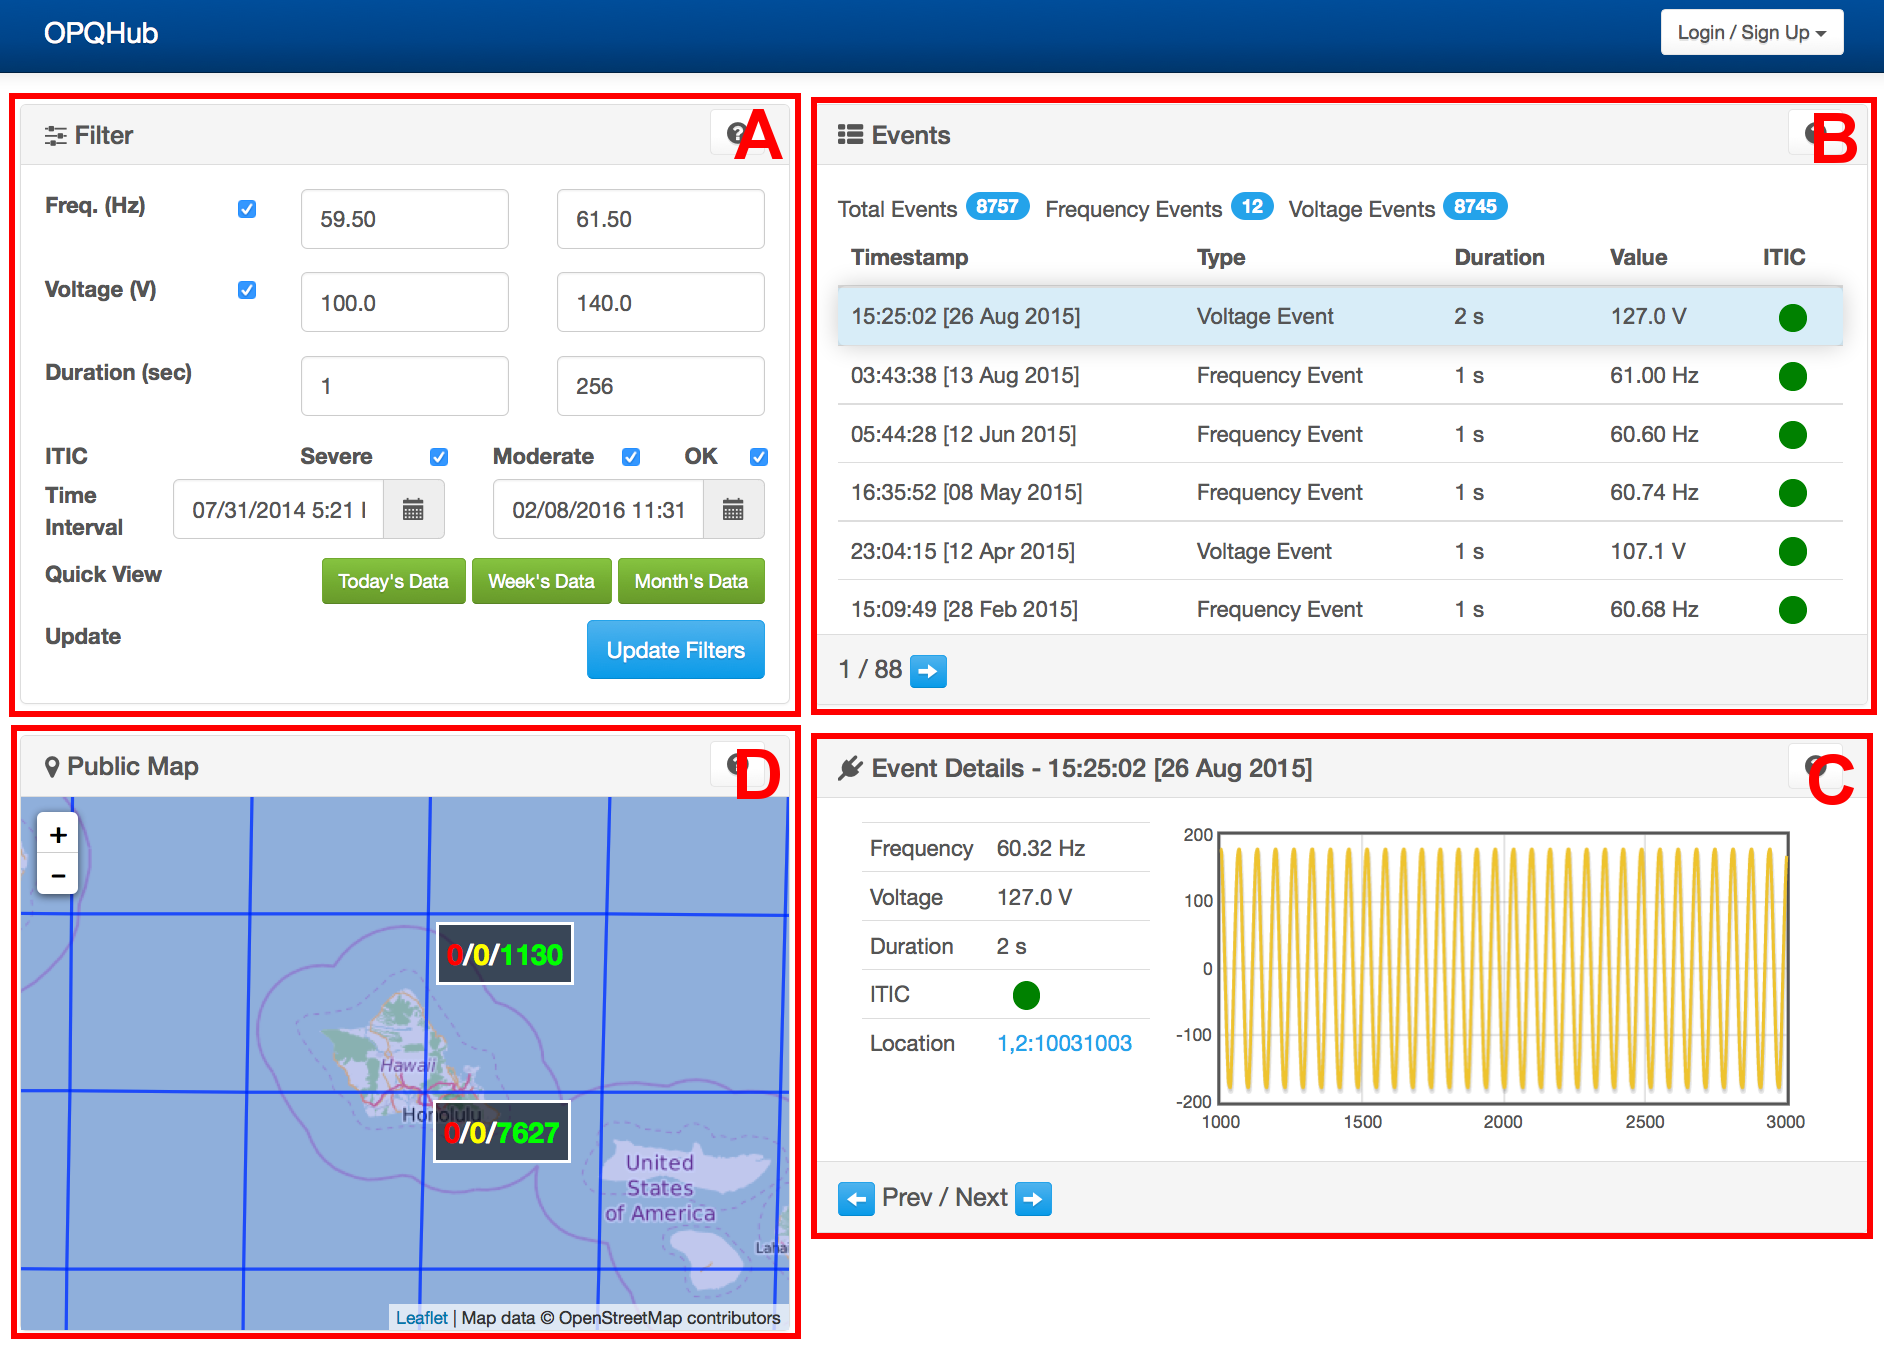
\includegraphics[width=\textwidth,height=13cm]{img/opqhub.png}
  \caption{OPQHub Distributed PQ Event and Information Reporting Interface. A) PQ events can be queried and filtered over complex criteria. B) List of PQ events that match filtered criteria. C) Details of a single PQ event. D) Dynamic map visualization of PQ events and query filter.}
  \label{fig:opqhub}
\end{figure*}

\subsection{Querying}
We provide facilities to query PQ events reported to our system by filtering on the following items: date, duration, min voltage, max voltage, min frequency, max frequency, severity as defined by the ITIC curve\cite{m:ITIC}, and location. Location queries are performed by using a bounding box given by the currently viewable area in a dynamic map interface.

A successful query returns a list of PQ events that meet the provided criteria. These events contain details about where and when the PQ event took place as well as raw waveform data that can be displayed using our interface.

\subsection{Quadtree Based Event Reporting}
A useful tool when working with any geographically distributed data set is a dynamic map to visualize events and other related information. We came across several issues when designing a map interface to display PQ events and information.

First, how can we maintain our users' privacy if a map displays the exact location of PQ events? We initially tried providing a randomization mechanism that would smudge the exact location randomly by some amount, but this didn't solve our second problem. Displaying multiple events generated by sensors that are close in time and location quickly clutter the map and reduced the amount of information available.

Building upon the open source map library Leaflet, we created a quadtree based grid visualization for displaying PQ events and related information that solves the issues related to users' privacy and multiple events being generated in the same location.

Instead of displaying PQ events as individual icons, the system utilizes GeoJson to display an aggregate count of events that are represented by the bounding box that forms a grid square. As the user zooms out, grids are combined together and the counts are combined into a more course grid layout. As the user zooms in, the grid squares are subdivided and the counts become more spread out and granular.

\subsubsection{Quadtree Based Grid Generation}
The top layer of our tree consists of a grid of squares where each square is 256 kilometers x 256 kilometers wide. Each top level grid square is then recursively subdivided into four squares of equals width. 

Our map was optimized to work with the state of Hawaii. Different parameters need to be chosen for using this map for other areas. For example, a larger state may require a courser or finer set of top level grid squares.

To generate an evenly spaced grid, we identified the NW and SE latitude and longitude points of the bounding box (BB) that contains the area of interest our grid should cover. The BB we chose for Hawaii is outlined in table \ref{tab:bb_hawaii}.

\begin{table}[htbp]
	\caption{Hawaii Grid Square Bounding Box}
	\label{tab:bb_hawaii}
	\begin{center}
		\begin{tabular}{|l|r|r|r|}
			\hline
			\textbf{BB Point} & \textbf{ Location} & \textbf{Latitude} & \textbf{Longitude}\\
			\hline
			North West & NW of Niihau & 22.534353 & -161.004639\\
			\hline
			South East & SE of Big Island & 16.719592 & -151.853027\\
			\hline
		\end{tabular} 
	\end{center}
\end{table}

We can calculate the latitude ($\phi$) and longitude ($\lambda$) of a point $(\phi_2, \lambda_2)$, given a starting point $(
\phi_1, \lambda_1)$, bearing ($\Theta$), distance ($d$), and angular distance ($AD=\frac{d}{radius\ of\ earth}$) with the following formula which uses the distance over a great arc circle as an approximation for the shape of the earth \cite{w:calc_lat_lng}.

$\phi_2 = asin(sin(\phi_1 * cos(AD) + cos(\phi_1) + sin(AD) * cos(\Theta))$

$\lambda_2 = \lambda_1 + atan2(sin(\Theta) * sin(AD) * cos(\phi_1), cos(AD) - sin(\phi_1) * sin(\phi_2))$

With the above formula, we start with the NW point of the BB, and generate all points due South of the starting point within the BB with a given distance interval. This process generates the first point for each of the row in our point matrix. Then for each starting point, we generate all points due East within the BB. The result of this process is a matrix of evenly spaced points which can then be used to create polygons of evenly spaced grid squares.

\subsubsection{Quadtree Based Geo-Hashing}
Our quadtree approach allows us to easily bin locations within a grid square at a given depth in the tree. Because of it's rigid structure, it's easy to use this data structure to perform geo-hashing of locations. The scheme we chose is as follows.

In order to associate OPQ hardware devices with locations on the grid, we developed a naming scheme that stores the parent information of each grid in the name itself. Grids at the coarsest grid scale (256 kilometers) are simply named by their row ($r$) and column ($c$) using the format $r,c:$. We show an example of how the coarsest grid squares would be named in figure \ref{fig:coarsest_grid_ids}.

\begin{figure}[htbp]
	\centering
	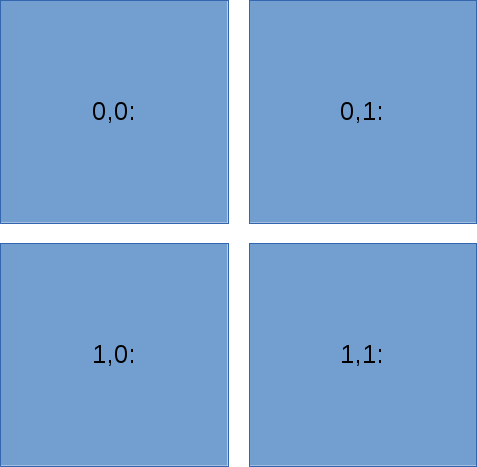
\includegraphics[width=0.6\columnwidth]{img/grid-sq.png}
	\caption{Naming Convention for Coarsest Grid Layer.}
	\label{fig:coarsest_grid_ids}
\end{figure}

For each level that the grid becomes more fine, each square recursively divides into four squares. We can name each of these child squares by its location in the parent square. For each finer level, we simply append this location id onto its parent's id.

\begin{table}[htbp]
	\caption{Naming of Child Grid Squares}
	\label{tab:grid_first_child}
	\begin{center}
		\begin{tabular}{|l|r|}
			\hline
			\textbf{Position in Parent} & \textbf{ID}\\
			\hline
			Top Left & 0\\
			\hline
			Top Right & 1\\
			\hline
			Bottom Right & 2\\
			\hline
			Bottom Left & 3\\
			\hline
		\end{tabular} 
	\end{center}
\end{table}

Figure \ref{fig:coarsest_grid_ids} shows the ids of the first level of children under the parent grid square.

%\begin{figure}[htbp]
%	\centering
%	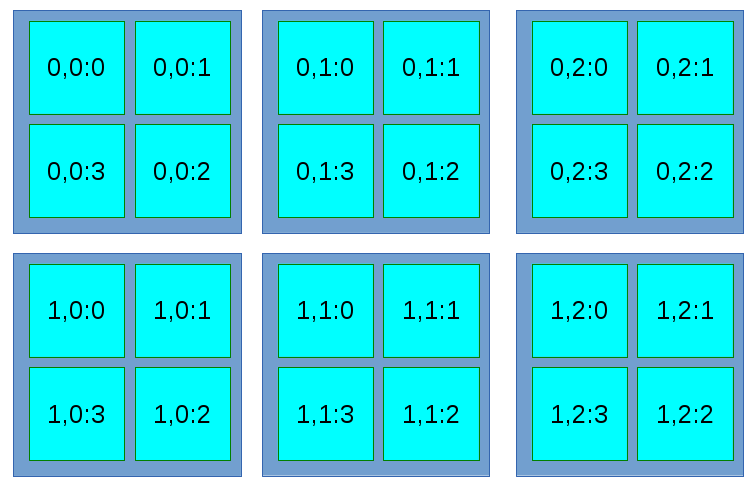
\includegraphics[width=0.8\columnwidth]{img/grid-sq-1.png}
%	\caption{Naming Convention for First Children.}
%	\label{fig:first_children}
%\end{figure}

We can then recursively use the same naming scheme for each level of children in the grid. For example, a grid id of ``0,0:13" represents the following information. At the coarsest level, the location ``0,0:" represents the top left 256x256 kilometer grid square. The following ``1" represents that the 128x128 kilometer child of the coarsest level is located at the top right of its parent square. The following ``3" represents that the grandchild of the coarsest square is in the bottom left of the child's square. To illustrate the concept of recursive ids, please refer to \ref{fig:second_children}.

\begin{figure}[htbp]
	\centering
	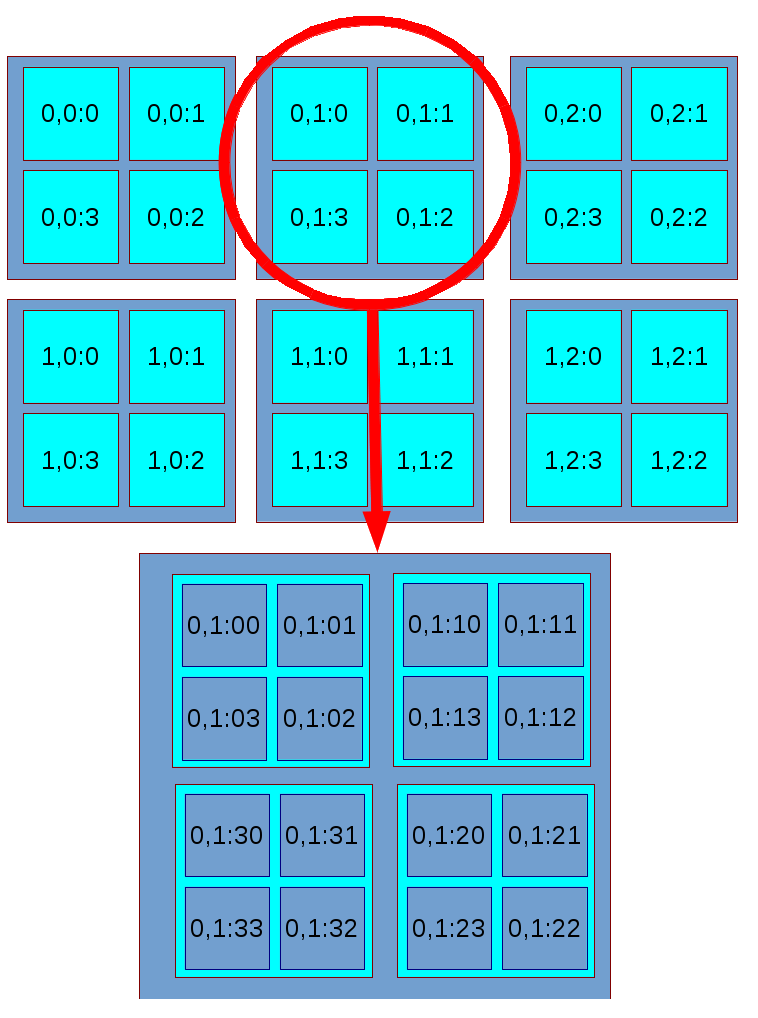
\includegraphics[width=0.8\columnwidth]{img/grid-sq-2.png}
	\caption{Recursive Naming of Children.}
	\label{fig:second_children}
\end{figure}

\begin{figure*}[htbp]
	\centering
	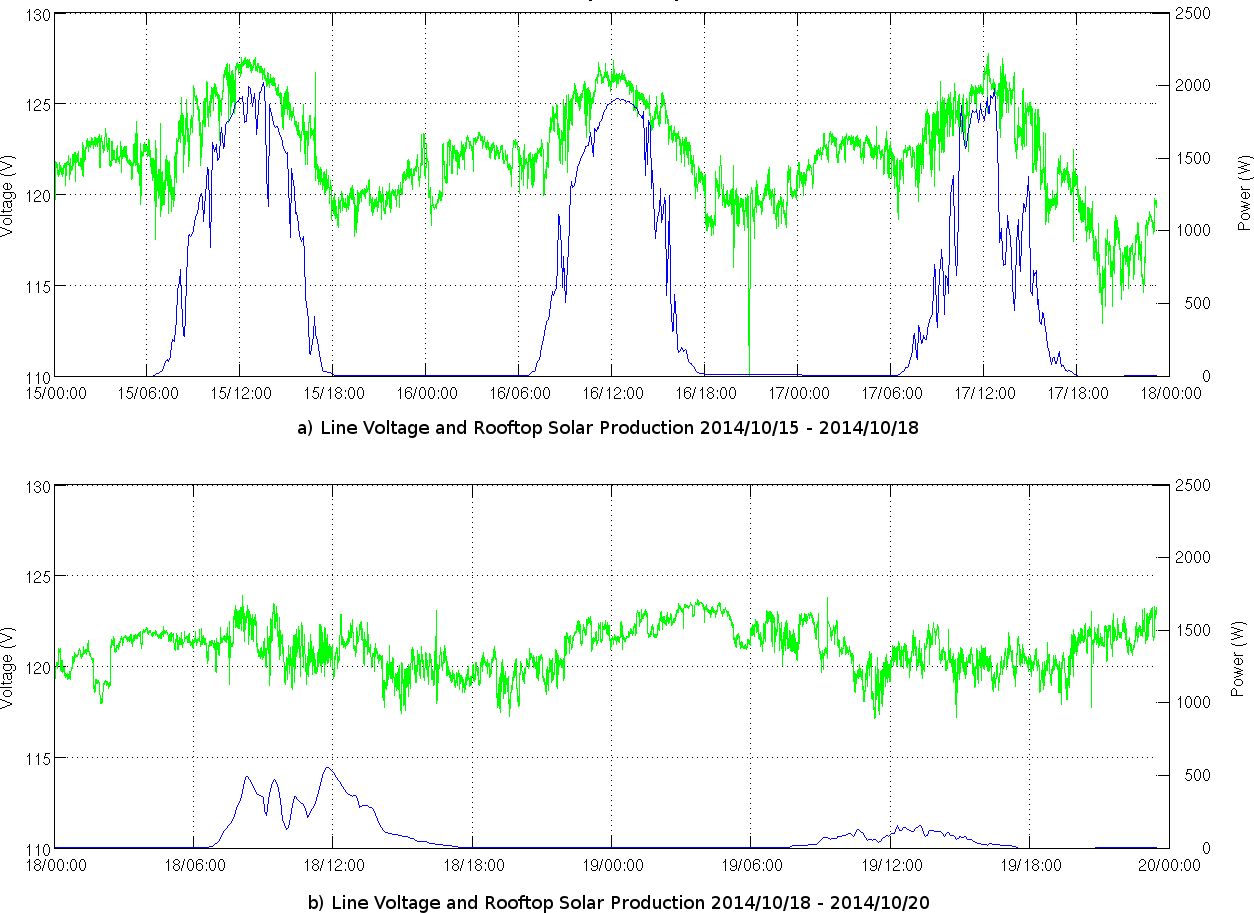
\includegraphics[width=0.8\textwidth]{img/weatherTrends.png}
	\caption{Top graph shows the residential line to neutral voltage and rooftop solar production during a sunny day on the Island of Oahu. Bottom graph shows the voltage and solar production during Hurricane Ana.}
	\label{fig:opqbox1}
\end{figure*}

\subsubsection{Dynamic Sizing of Grid}
Grid scale is defined as the length of each square polygon in the grid. That is, a grid scale of 256 kilometers contains grid squares which each are 256 kilometers by 256 kilometers. The coarsest grid scale that we support is 256 kilometers and the finest grid scale is $\frac{1}{8}$ kilometer.

We designed our grid-map library so that when the map is zoomed out, it displays the coarsest grid of 256 kilometers. As the map is zoomed in, each grid square is recursively divided into four smaller squares, each with a grid-scale that is exactly one-half of its parent's. This process continues until the map is at max zoom and each grid square represents $\frac{1}{8}$ of a kilometer.

The location of any grid is invariant to both zoom and pan as long as the NE BB starting point is not changed. This makes it easy to associate ids with individual grid squares so that devices can then be associated with individual grid squares.

\subsubsection{Privacy Gained From Quadtree Approach}
If a user decides to include their location, they are able to select a grid square at a depth that they are comfortable and that describes their location. If a user is not as concerned about their privacy, they can select a grid square that might enclose their house. If a user is more privacy conscious, they might select a grid square that contains their block, their neighborhood, or an entire island. We empower our users to select a coarseness of location which suits their privacy needs.







\section{Pilot}
Distributed PQ monitoring is a common subject in literature\cite{daponte2004transientmeter}\cite{byman2000using}\cite{cristaldi2002distributed}. Projects such as F-NET\cite{zhang2010wide} have demonstrated the utility of Phaser Measurement Unit in monitoring of the US power grid. Distributed PQ recorders such as PQube\cite{von2014micro} have been used in many research applications, from renewable integration, to novel smartgrid designs.

Dense distributed consumer level monitoring, on the order of a meter for $10mi^2$ is not often considered due to cost, privacy, and bandwidth constraints. 

\subsection{OPQBox}

In order to demonstrate our privacy enabled grid visualization method, we developed and deployed five in-house built power quality monitors (OPQBox1). OPQBox1 connects to the user's power outlet, via a step-down transformer and digitizes the resulting signal. While the sampling was controlled by a real-time MCU, waveform analysis was performed by the Raspberry Pi SBC. OPQBox1 computed average frequency and line to neutral voltage at 1 second intervals. By connecting to the resident's 802.11 WIFI, OPQBox1 forwarded both the raw digitized signal as well as the computed frequency and RMS voltage to OPQHub for display. OPQBox1 lacked GPS and used NTP for synchronization. 

\subsection{Deployment}

Five OPQBox1 devices were deployed as a part of an OPQHub pilot study. Two devices were located in residential housing,  two in an apartment building, and one in an office building. As part of the privacy enabled visualization only the office building's location was set in the OPQHub. Devices located in the apartment building were located to the 250mx250m grid square at depth five in the quad tree. Similarly, devices located in houses were constrained to the 500mx500m grid square at the quad tree depth of 4. 

If the frequency or voltage recorder by the OPQBox1 was outside of a set threshold, OPQHub would mark a 1 second measurement as an event if:
\begin{itemize}
\item Frequency deviated by $\pm 0.5Hz$ from the $60Hz$.
\item RMS voltage deviated by $\pm 7V_{rms}$ from the $120V_{rms}$.
\end{itemize}
Voltage events were further classified by severity using the ITIC Curve standard\cite{m:ITIC}. Over 10000 events were recorded, 30 of those events were categorized as an ITIC interruption and 2 were in the prohibited region. However, these events were localized to an individual device. This leads us to believe that the disturbance originated from the consumer's side of the meter. Only 12 events were temporally correlated between multiple devices. An example of such event is shown in Figure \ref{fig:gridwide}. 

\begin{figure}[htbp]
	\centering
	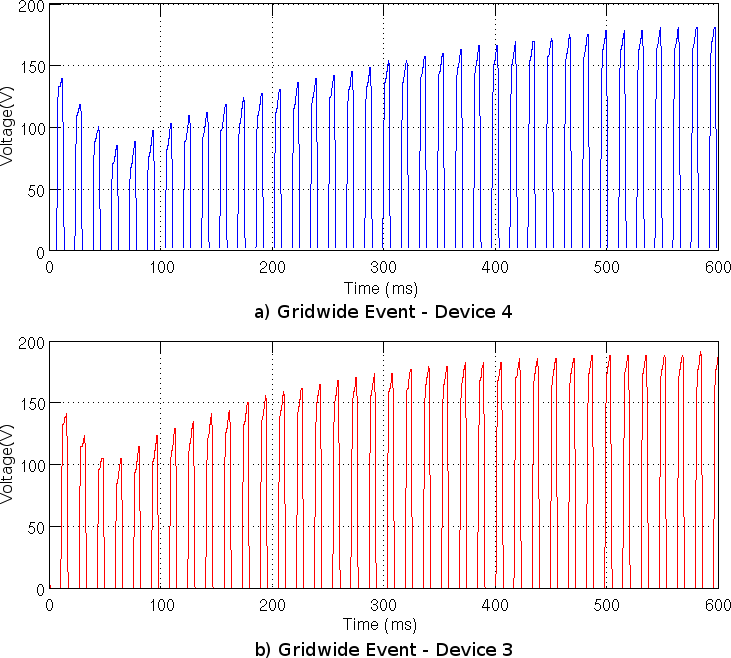
\includegraphics[width=1\columnwidth]{img/gridwide.png}
	\caption{Event recorded by two devices. Only positive voltage is displayed for clarity.}
	\label{fig:gridwide}
\end{figure}

As a part of our pilot study we considered integration of the renewable generation data into OPQHub. Figure \ref{fig:opqbox1} shows the neutral-line voltage trend in green and rooftop solar production in blue. Its worth noting that the the OPQBox1 device which recorded this trend was located in a residential house, 20 miles away from the rooftop solar installation. The first plot in Figure \ref{fig:opqbox1} shows the OPQBox1 recorded voltage in green as well as the solar power production as reported by the Enphase\textregistered {} inverter. During October 15-18 2014, with typical sunny weather, line voltage tracks solar production. During October 18-20, however hurricane Ana passed within 100mi from the island of Oahu. With almost complete cloud cover, rooftop solar production was diminished, and the daily voltage swell was not observed. It is our aim to integrate inverter readings into OPQHub on an opt-in basis.



\section{Conclusion \& Future Work}
We developed an open source software and hardware framework for visualizing PQ events and information while maintaining users’ privacy. We performed a pilot study on both our hardware and software by deploying sensors across Oahu and aggregating and visualizing data using OPQHub. Our pilot study showed strong correlations between PV output and voltage fluctuations. We showed several severe events that were localized to a household and not a grid wide event. This indicates that our framework can differentiate between localized and grid-wide PQ events.

In the next version of OPQHub we intend to solidify our privacy controls by providing the ability to share data with trusted partners by adding the ability to define collections of OPQBoxes that provide specific privacy controls on those collections. Thus, users will be able to control their privacy at the individual level and at the level of groups of individuals.  Further, we intend to make a fully reactive user-interface for filtering and querying, build upon our grid based interface, and support a larger selection of PQ event types. Our next PQ meter OPQBox2 aims to be IEEE 1159 compliant, with optional GPS synchronization, and battery backup. 


\bibliographystyle{IEEEtran}
\bibliography{refs}

\end{document}


